\documentclass[11pt]{article}
\usepackage{scrtime} % for \thistime (this package MUST be listed first!)
\usepackage{graphicx}
\usepackage{float}
\usepackage[margin=0.75in]{geometry}
\usepackage{fancyhdr}
\usepackage{caption}
\usepackage[backend=bibtex, giveninits=true, doi=false, isbn=false, natbib=true, url=false, eprint=false, style=authoryear, sorting=nyt, maxcitenames=2, maxbibnames=10, minbibnames = 10, uniquename=false, uniquelist=false, dashed=false]{biblatex} % can change the maxbibnames to cut long author lists to specified length followed by et al., currently set to 99.
%% bibliography for each chapter...
\DeclareFieldFormat[article,inbook,incollection,inproceedings,patent,thesis,unpublished]{title}{#1\isdot} % removes quotes around title
\renewbibmacro*{volume+number+eid}{%
	\printfield{volume}%
	%  \setunit*{\adddot}% DELETED
	\printfield{number}%
	\setunit{\space}%
	\printfield{eid}}
\DeclareFieldFormat[article]{number}{\mkbibparens{#1}}
%\renewcommand*{\newunitpunct}{\space} % remove period after date, but I like it. 
\renewbibmacro{in:}{\ifentrytype{article}{}{\printtext{\bibstring{in}\intitlepunct}}} % this remove the "In: Journal Name" from articles in the bibliography, which happens with the ynt 
\renewbibmacro*{note+pages}{%
	\printfield{note}%
	\setunit{,\space}% could add punctuation here for after volume
	\printfield{pages}%
	\newunit}   
\DeclareFieldFormat{journaltitle}{#1\isdot} 
\DefineBibliographyStrings{english}{% clears the pp from pages
	page = {\ifbibliography{}{\adddot}},
	pages = {\ifbibliography{}{\adddot}},
} 
\DeclareNameAlias{sortname}{last-first}
\renewcommand*{\revsdnamepunct}{}%remove comma between last name and first name
\renewcommand*{\nameyeardelim}{\addspace} % remove comma in text between name and date
%\addbibresource{C:/Users/synch/Documents/Bib/Gene_expression2.bib} % The filename of the bibliography
%\addbibresource{C:/Users/synch/Documents/Bib/Gene_expression2.bib} % The filename of the bibliography
\usepackage[autostyle=true]{csquotes} % Required to generate language-dependent quotes in the bibliography
\renewrobustcmd*{\bibinitperiod}{}
% you'll have to play with the citation styles to resemble the standard in your field, or just leave them as is here. 
% or, if there is a bst file you like, just get rid of all this biblatex stuff and go back to bibtex. 


%\usepackage[round]{natbib}
%\setcitestyle{aysep={}} %removes the comma between the author and year in citations
\usepackage[hidelinks]{hyperref} %hidelinks will remove ugly coloured links in the text
%\usepackage{underscore}
\usepackage{pdfpages}
\usepackage{xcolor,colortbl}%for changing cell colour
\usepackage{multirow}
\usepackage[normalem]{ulem}
\useunder{\uline}{\ul}{}
\usepackage{xspace}
\usepackage{longtable}
\usepackage{booktabs}
\usepackage{capt-of}
\pagestyle{fancy}
\setlength{\headheight}{15.2pt}
\setlength{\headsep}{13 pt}
\setlength{\parindent}{28 pt}
\setlength{\parskip}{12 pt}
\pagestyle{fancyplain}
\usepackage[T1]{fontenc}
\usepackage{tikz-cd}
\usepackage{color,amsmath,amssymb,amsthm,mathrsfs,amsfonts,dsfont}
\usepackage{xspace}
\usepackage{tikz-cd}
\usepackage{tikz}
\usetikzlibrary{decorations.markings}
\usetikzlibrary{calc, arrows}
\usepackage{longtable}
\usepackage{xcolor,colortbl}%for changing cell colour\usepackage[hidelinks]{hyperref} %hidelinks will remove ugly coloured links in the text
%\usepackage{caption}
%\usepackage{subcaption}
\usepackage{multicol}
%\usepackage[round]{natbib}
%\usepackage[demo]{graphicx}
\usepackage{subfig}\usepackage{subfig}% http://ctan.org/pkg/subfig
\usepackage{tabularx}
\lhead{}
%\rhead{Daniella Lato \thepage\ }
\rhead{Daniella F Lato and G Brian Golding}
\title{\sc Spatial Patterns of Gene Expression in Bacterial Genomes}
\author{\sc Daniella F Lato\textsuperscript{1} and G Brian Golding\textsuperscript{1}* \\ \sc Paper Draft}
%\date{\sc Committee Members: \\ \sc Dr. Brian Golding \\ \sc Dr. Marie Elliot \\ Transfer Exam Chair: \\ Dr. Ben Evans}
\renewcommand\headrulewidth{0.5mm}

%below 3 lines will put ALL table captions at the top...not sure if this is what we want but it is good enough for now
\usepackage{float}
\floatstyle{plaintop}
\restylefloat{table}
%%%%%%%%%%%%%%%%%%%%%%%%%%%%%%%%%%%%%%%%%%%%%%%%%%%%%%%%%%%%%%%%%%%
\usepackage{graphicx}
\usepackage{float}
\usepackage[margin=0.75in]{geometry}
\usepackage{fancyhdr}
\usepackage{caption}
\usepackage[super]{natbib}
\usepackage[hidelinks]{hyperref} %hidelinks will remove ugly coloured links in the text
\usepackage{pdfpages}
\usepackage{xcolor,colortbl}%for changing cell colour
\usepackage{multirow}
\usepackage[normalem]{ulem}
\usepackage{xspace}
\usepackage{longtable}
\usepackage{booktabs}
\usepackage{capt-of}
\pagestyle{fancy}
\setlength{\headheight}{15.2pt}
\setlength{\headsep}{13 pt}
\setlength{\parindent}{28 pt}
\setlength{\parskip}{12 pt}
\pagestyle{fancyplain}
\usepackage[T1]{fontenc}
\usepackage{tikz}
\usepackage{tikz-cd}
\usepackage{color,amsmath,amssymb,amsthm,mathrsfs,amsfonts,dsfont}
\lhead{Stats744}
\rhead{Daniella Lato}
\renewcommand\headrulewidth{0.5mm}
\usepackage{setspace}
\usepackage{multirow}

\begin{document}
	\begin{figure*}[t!]
		\centering{
			\resizebox{\textwidth}{!}{%
				\begin{tikzpicture}[x=1in, y=1in]
				%circle on left
				\draw[line width=0.7mm,
				decoration={markings, 	
					%the position below denotes the distance from the right most point of the circle (3 on a clock) going counter clock wise 1= 3oclock position
					%arrow for "replication" direction
					mark=at position 0.2 with {\arrow[>=angle 45]{<}},
					%oriC tick
					mark=at position 0.0513 with {\arrow[line width=0.7mm]{|}},
					%oriC node
					mark=at position 0.049 with \node[above right](ori){\textit{oriC} (20bp)};,
					%10bp tick
					mark=at position 0.15 with {\arrow[line width=0.7mm]{|}},
					%position 90 tick
					mark=at position 0.35 with {\arrow[line width=0.7mm]{|}},
					%position 0/100 tick
					mark=at position 0.25 with {\arrow[line width=0.7mm]{|}},
					%position 0/100 node
					mark=at position 0.25 with \node[above](pos0){1bp/100bp};,
					%80bp tick
					mark=at position 0.45 with {\arrow[line width=0.7mm]{|}},			
					%80bp node
					mark=at position 0.45 with \node[above left](pos80){80bp};,
					%70bp tick
					mark=at position 0.55 with {\arrow[line width=0.7mm]{|}},
					%ter tick
					mark=at position 0.65 with {\arrow[line width=0.7mm]{|}},		
					%ter node lab
					mark=at position 0.648 with \node[](ter){};,
					%ter node lab
					mark=at position 0.69 with \node[below left]{\textit{ter} (60bp)};,
					%30bp tick
					mark=at position 0.95 with {\arrow[line width=0.7mm]{|}},
					%40bp tick
					mark=at position 0.85 with {\arrow[line width=0.7mm]{|}},
					%40bp node
					mark=at position 0.85 with \node[below right](pos40){40bp};,
					%50bp tick
					mark=at position 0.75 with {\arrow[line width=0.7mm]{|}},
				},
				postaction={decorate}] (1.5,1.5) circle (1in);
				%arrow between circles
				\draw[->,line width=0.7mm, >=triangle 45] (3,1.5) -- (4,1.5);
				%line btwn origin and middle of circle
				\draw[line width=0.7mm, dashed] (1.5,1.5) -- (ori);
				%line btwn ter and middle of circle
				\draw[line width=0.7mm, dashed] (1.5,1.5) -- (ter);
				%circle to the right
				\draw[line width=0.7mm,
				decoration={markings, 	
					%the position below denotes the distance from the right most point of the circle (3 on a clock) going counter clock wise 1= 3position
					%arrow for "replication" direction #1
					mark=at position 0.125 with {\arrow[>=angle 45]{>}},
					%oriC tick
					mark=at position 0.053 with {\arrow[line width=0.7mm]{|}},
					%oriC node
					mark=at position 0.05 with \node[above right](ori2){\textit{oriC} (1bp)};,
					%position 90 tick
					mark=at position 0.35 with {\arrow[line width=0.7mm]{|}},
					%40 tick
					mark=at position 0.45 with {\arrow[line width=0.7mm]{|}},
					%position 40 node
					mark=at position 0.45 with \node[above left](2pos80){40bp};,
					%position 0/100 tick
					mark=at position 0.25 with {\arrow[line width=0.7mm]{|}},
					%position 0/100 node
					mark=at position 0.25 with \node[above](2pos0){20bp};,
					%10 tick
					mark=at position 0.15 with {\arrow[line width=0.7mm]{|}},	
					%ter node lab
					mark=at position 0.70 with \node[below left](ter2){\textit{ter} (60bp/40bp)};,
					%ter node
					mark=at position 0.648 with \node[](terr){};,
					%50 tick
					mark=at position 0.55 with {\arrow[line width=0.7mm]{|}},
					%ter tick
					mark=at position 0.65 with {\arrow[line width=0.7mm]{|}},
					%position 40 tick
					mark=at position 0.85 with {\arrow[line width=0.7mm]{|}},
					%30 tick
					mark=at position 0.95 with {\arrow[line width=0.7mm]{|}},
					%50 tick
					mark=at position 0.75 with {\arrow[line width=0.7mm]{|}},
					%40 node
					mark=at position 0.85 with \node[below right](2pos40){20bp};,
					%arrow for "replication" direction #2
					mark=at position 0.995 with {\arrow[>=angle 45]{<}}
				},
				postaction={decorate}] (5.5,1.5) circle (1in);
				%line btwn origin and middle of circle
				\draw[line width=0.7mm, dashed] (5.5,1.5) -- (ori2);
				%line btwn ter and middle of circle
				\draw[line width=0.7mm, dashed] (5.5,1.5) -- (terr);
				%fig lable A
				\node[] at (0.2,0.15) {\LARGE \textbf{(A)}};
				%fig lable B
				\node[] at (4.2,0.15) {\LARGE \textbf{(B)}};
				\end{tikzpicture}
			}%resiebox
		}
		\caption{\label{originScaling} Schematic of the transformation used to scale the positions in the genome to the origin of replication and account for bidirectional replication. Circle (A) represents the original replicon genome without any transformation. Circle (B) represents the same replicon genome after the transformation. The origin of replication is denoted by ``\textit{oriC}'' and the terminus of replication is denoted by ``\textit{ter}''. The dashed line represents the two halves of the replicon separate by replication. The replicon genome in this example is 100 base pairs in length. Every 10 base pairs is denoted by a tick on the genome. The origin in (A) is at position 20 in the genome and is transformed in (B) to become position 1. The terminus is at position 60 in (A) and position 60 and 40 in (B). The terminus has two positions in (B) depending on which replicon half is being accounted for.
			If the replication half to the right of the origin is considered, the terminus will be at position 40.
			If the replication half to the left of the origin is considered, the terminus will be at position 60.
			Position 40 in (A) becomes position 20 in (B). Position 80 in (A) becomes position 40 in (B), because of the bidirectional nature of bacterial replication.}\vspace*{1pt}
	\end{figure*}
	
	
\end{document}
